\documentclass[12pt, a4paper]{report}
\usepackage[top=1.0in, bottom=1.0in, left=0.8in, right=0.8in]{geometry}

\setlength{\parskip}{\baselineskip}%
\setlength{\parindent}{0pt}%
\usepackage[]{graphicx}
\usepackage{enumitem}
\usepackage{amsmath}
\usepackage{relsize}
\usepackage{cprotect}
\usepackage{amsmath, amsfonts}
\usepackage{siunitx}
\usepackage{mathrsfs}
\usepackage{framed}
\usepackage{enumitem}
\usepackage{tikz}
\usepackage{circuitikz}
\usepackage{float}
\usepackage[english]{babel}
\usepackage{blindtext}

\hyphenpenalty=10000

\newlist{notes}{enumerate}{1}
\setlist[notes]{label=\textbf{Note:} ,leftmargin=*}

\newlist{hints}{enumerate}{1}
\setlist[hints]{label=\textbf{Hint:} ,leftmargin=*}

\usepackage{xcolor}
\usepackage{color}
\definecolor{com1}{RGB}{125,125,125}
\definecolor{comment}{RGB}{140,115,115}
\definecolor{numbering}{rgb}{0.2,0.2,0.2}
\definecolor{key}{RGB}{0,0,180}
\definecolor{in}{RGB}{0,100,0}
\definecolor{out}{RGB}{100,30,30}
\definecolor{bg}{RGB}{245,245,245}
\definecolor{bgLight}{RGB}{250,250,250}
\definecolor{string}{RGB}{0,150,0}

\usepackage{hyperref}
\hypersetup{
    colorlinks=true,
    linkcolor=blue,
    filecolor=magenta,      
    urlcolor=blue,
}
\urlstyle{same}

\usepackage{listings}

\lstdefinestyle{py_code}{ %
    backgroundcolor=\color{bg},      % choose the background
    basicstyle=\ttfamily\small,		      % fonts
    breakatwhitespace=false,         % automatic breaks at whitespace ?
    breaklines=true,                 % sets automatic line breaking
    captionpos=b,                    % caption-position - bottom
    commentstyle=\itshape\color{comment},    % comment style
    extendedchars=true,              % use non-ASCII
    frame=single,	                   % single frame around the code
    keepspaces=true,                 % keeps spaces in text
    keywordstyle=\bfseries\color{key},% keyword style
    language=Python,                 	  % the language of the code
    morekeywords={Null},       % add more keywords to the set
    numbers=left,                    % line_numbers (none, left, right)
    numbersep=10pt,                  % line_no - code dist
    numberstyle=\footnotesize\color{numbering}, % line_no style
    rulecolor=\color{black},         % frame_color [!always set]
    showspaces=false,                % show spaces everywhere
    showstringspaces=false,          % 
    showtabs=false,                  % 
    stepnumber=1,                    % step b/w two line-no
    stringstyle=\color{string},     % string literal style
    tabsize=2,	                       % sets default tabsize to 2 spaces
    title=\lstname,                  % show the filename
    escapeinside={(*}{*)},			  % escape from style inside (* *)
    xleftmargin=\parindent,
    belowskip=-1.3 \baselineskip,
    aboveskip=1.0 \baselineskip,
    columns=fullflexible,
    xleftmargin=0.15in,
}
\lstnewenvironment{py_code}
{\lstset{style=py_code}}
{}

\lstdefinestyle{psudo}{ %
    backgroundcolor=\color{bgLight},   % choose the background
    basicstyle=\ttfamily\small,		      % fonts
    breakatwhitespace=false,         % automatic breaks at whitespace ?
    breaklines=true,                 % sets automatic line breaking
    captionpos=b,                    % caption-position - bottom
    commentstyle=\itshape\color{com1},          % comment style
    extendedchars=true,              % use non-ASCII
    keepspaces=true,                 % keeps spaces in text
    language=C,                 	  % the language of the code
    morekeywords={type,NULL, True, False},       % add more keywords to the set
    showspaces=false,                % show spaces everywhere
    showstringspaces=false,          % 
    showtabs=false,                  % 
    tabsize=2,	                       % sets default tabsize to 2 spaces
    title=\lstname,                  % show the filename
    escapeinside={(*}{*)},			  % escape from style inside (* *)
    belowskip=-1.8 \baselineskip,
    aboveskip=0.9 \baselineskip,
    columns=fullflexible,
    xleftmargin=0.2in,
    frame=tb,
    framexleftmargin=16pt,
    framextopmargin=6pt,
    framexbottommargin=6pt, 
    framerule=0pt,
}

\lstnewenvironment{psudo}
{\lstset{style=psudo}}
{}

\graphicspath{ ./ }


\title{\textf{EE2703 : Applied Programming Lab \\ Assignment 3 \\ Fitting Data to Models}} 
\author{Saurav Sachin Kale \\ EE19B141} % Author name

\date{\today} % Date for the report

\begin{document}		
		
\maketitle % Insert the title, author and date

\section*{Aim}
The aim of this assignment is to
\begin{itemize}
  	\item Process data with noise
  	\item Perform curve fitting to fit the data to the mathematical model
	\item Study the effect of noise on curve fitting by analysing error in the calculation of the coefficients in the mathematical expression for varying amounts of noise
 \end{itemize}

\section*{Procedure}
\begin{description}[font=$\bullet$]
\item On running ``generate\_data.py'' (kindly ensure the python file and fitting.dat are in same directory) a set of data points are generated in the file ``fitting.dat" for the equation 
\begin{equation}\label{eq:1}
f(t)=1.05J_{2}(t)-0.105t+n(t)
 \end{equation}
\\
where $n(t)$ is the amount of noise.  The noise is given to be normally distributed, i.e., its probability distribution is given by
 \begin{equation*}
\mathrm{P}(n(t)|\sigma)=\frac{1}{\sigma\sqrt{2\pi}}\text{exp}\left(-\frac{n(t)^{2}}{2\sigma^{2}}\right)
 \end{equation*}
with $\sigma$, the standard deviation of noise given by
\begin{psudo}
sigma=logspace(-1,-3,9)
\end{psudo}
\\
logspace is a python function which returns number spaces evenly in interval on a log scale.
\\
The first column in data points file "fitting.dat" has the value of $t$.
\item Our mathematical model for this data is:
\begin{equation}\label{eq:2}
g(t;A,B)=AJ_{2}(t)+Bt
\end{equation}
$A$ and $B$ are to be found so as to fit this curve to our data points.
\item The true values of $A$ and $B$ are:
\begin{equation*}
    A = 1.05, B = -0.105
\end{equation*}
\item The equation (2) can be interpreted as a matrix product in the following manner:
\begin{equation}
g(t;A,B)=
    \begin{pmatrix}
J_{2}(t_{1}) & t_{1}\\
... & ... \\
J_{2}(t_{m}) & t_{m}
\end{pmatrix}
\cdot
\begin{pmatrix}
A\\B
\end{pmatrix}
=M\cdot p
\end{equation}
\item $M$ contains the values of $J_2(t)$ and the corresponding $t$ values. $p$ concists of the coefficients $A$ and $B$
\item Now we can find $A$ and $B$ by taking the mean squared error as follows:
\begin{equation}
\epsilon_{ij}=\frac{1}{101}\sum_{k=0}^{101}\left(f_{k}-g(t;A,B)\right)^{2}
\end{equation} 
\item Plotting a contour plot of $\epsilon_{ij}$ vs. $A$ and $B$ and finding those values of $A$ and $B$ for which Error $ \longrightarrow 0$ gives the estimate of those values of $A$ and $B$ which fit the curve approximately to the data points.
\item This estimate is found using the method of least squares. The python function below from the SciPy library is used:
\begin{psudo}
scipy.linalg.lstsq(M,p)
\end{psudo}
(uses the method of least squares to find estimates of $A$ and $B$)
\begin{figure}[H]
	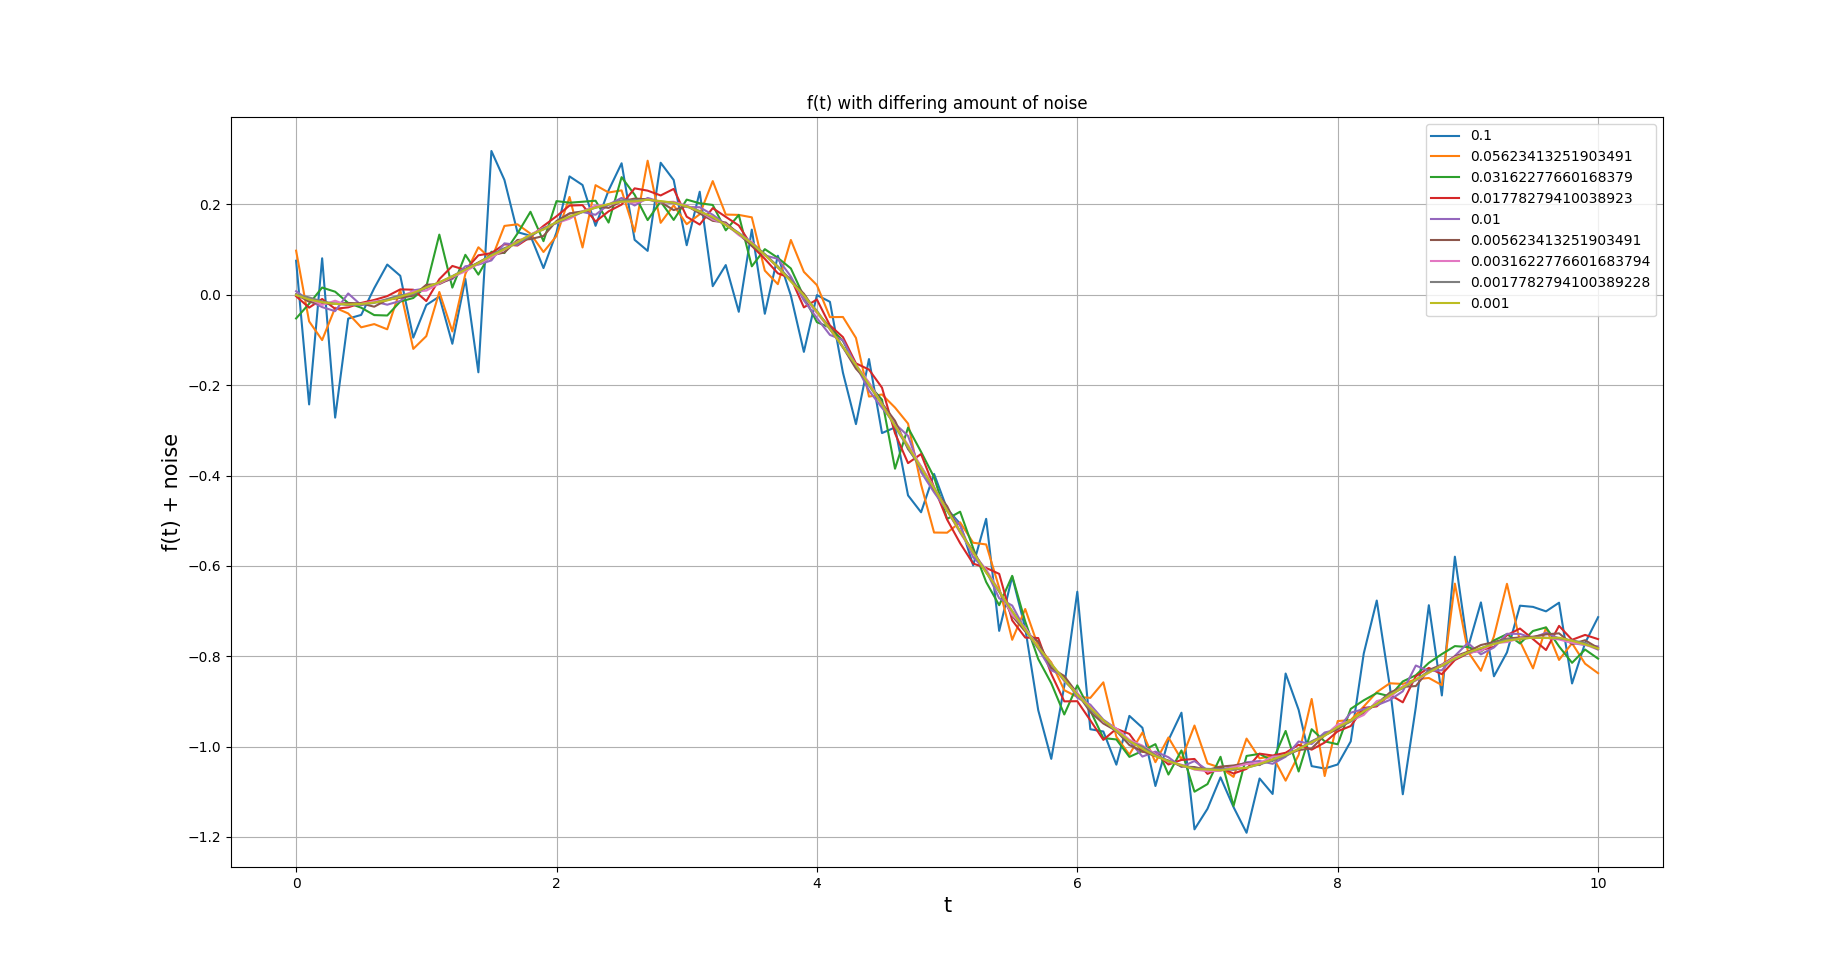
\includegraphics[scale=0.35]{Figure_1.png} 
	\caption{Plot of generated data to fit}
	\label{fig:rawdata}
\end{figure}
\end{description}


\subsection*{Results}
\begin{enumerate}
\item The plot of the data to be fitted with true curve highlighted:
\begin{figure}[H]
	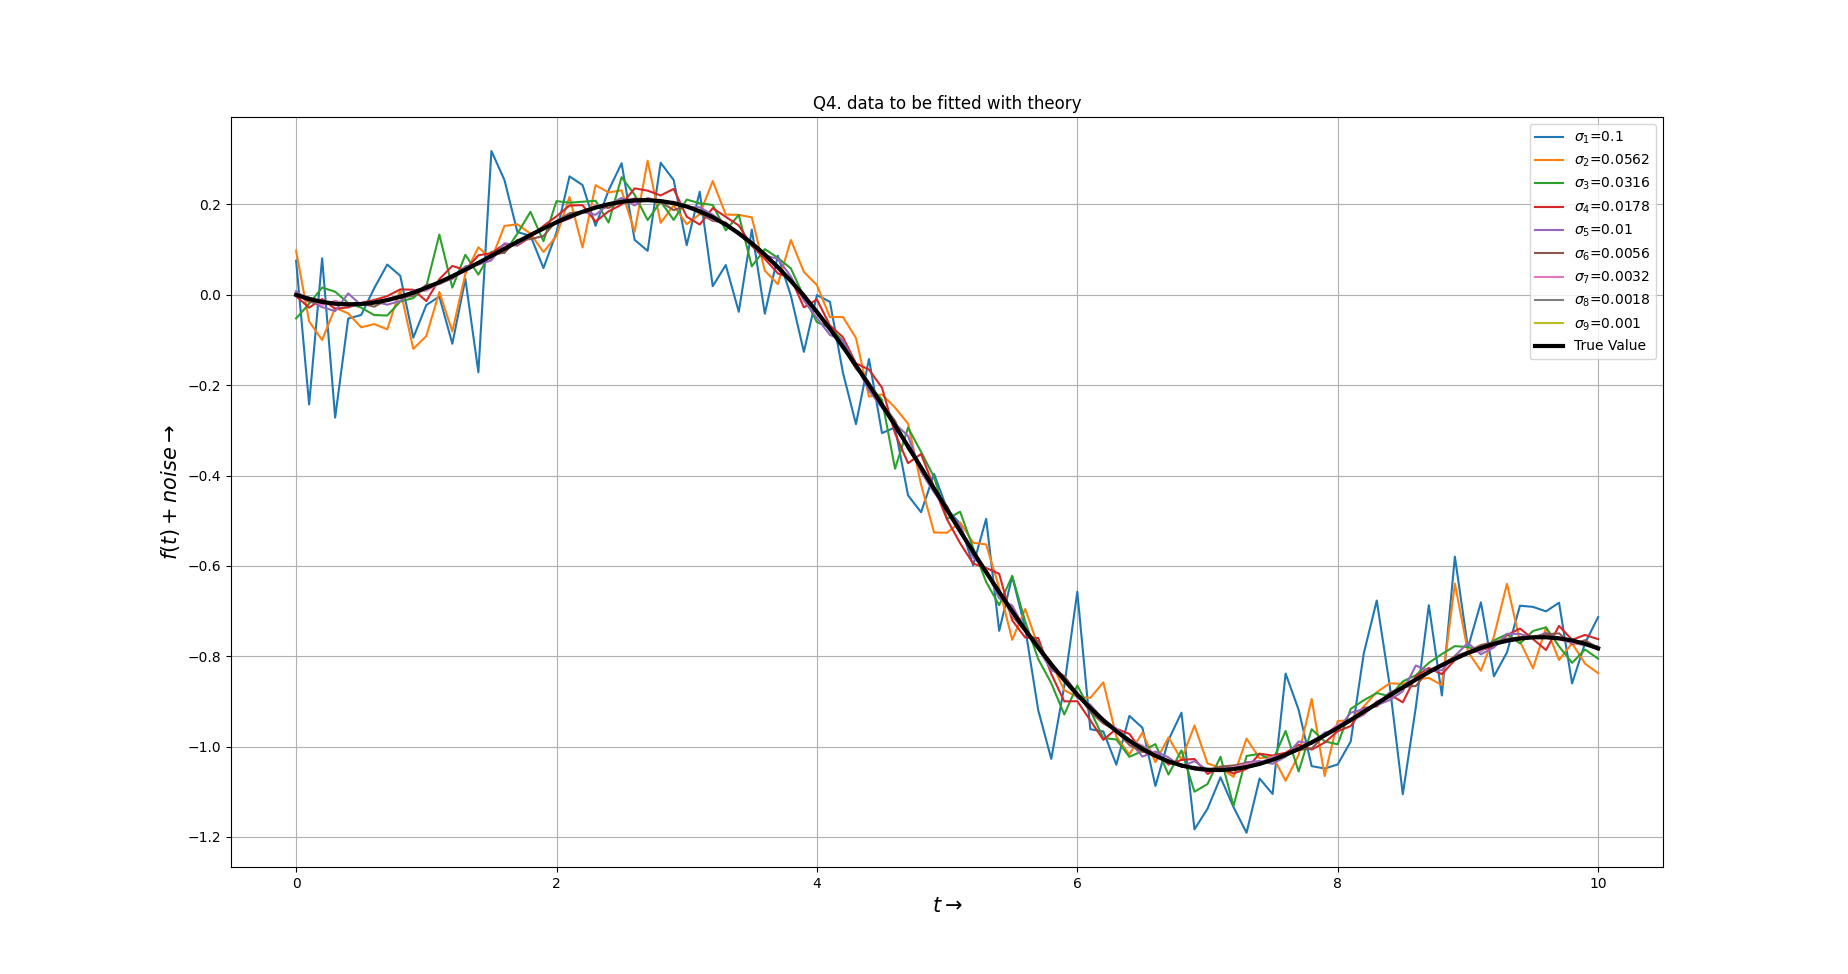
\includegraphics[scale=0.35]{Figure_2.png} 
	\caption{Plot of generated data and the true curve}
	\label{fig:rawdata}
\end{figure}

\clearpage

\item Errorbar plot shows the deviation from the true value for noise whose standard deviation is 0.1 
\begin{figure}[H]
	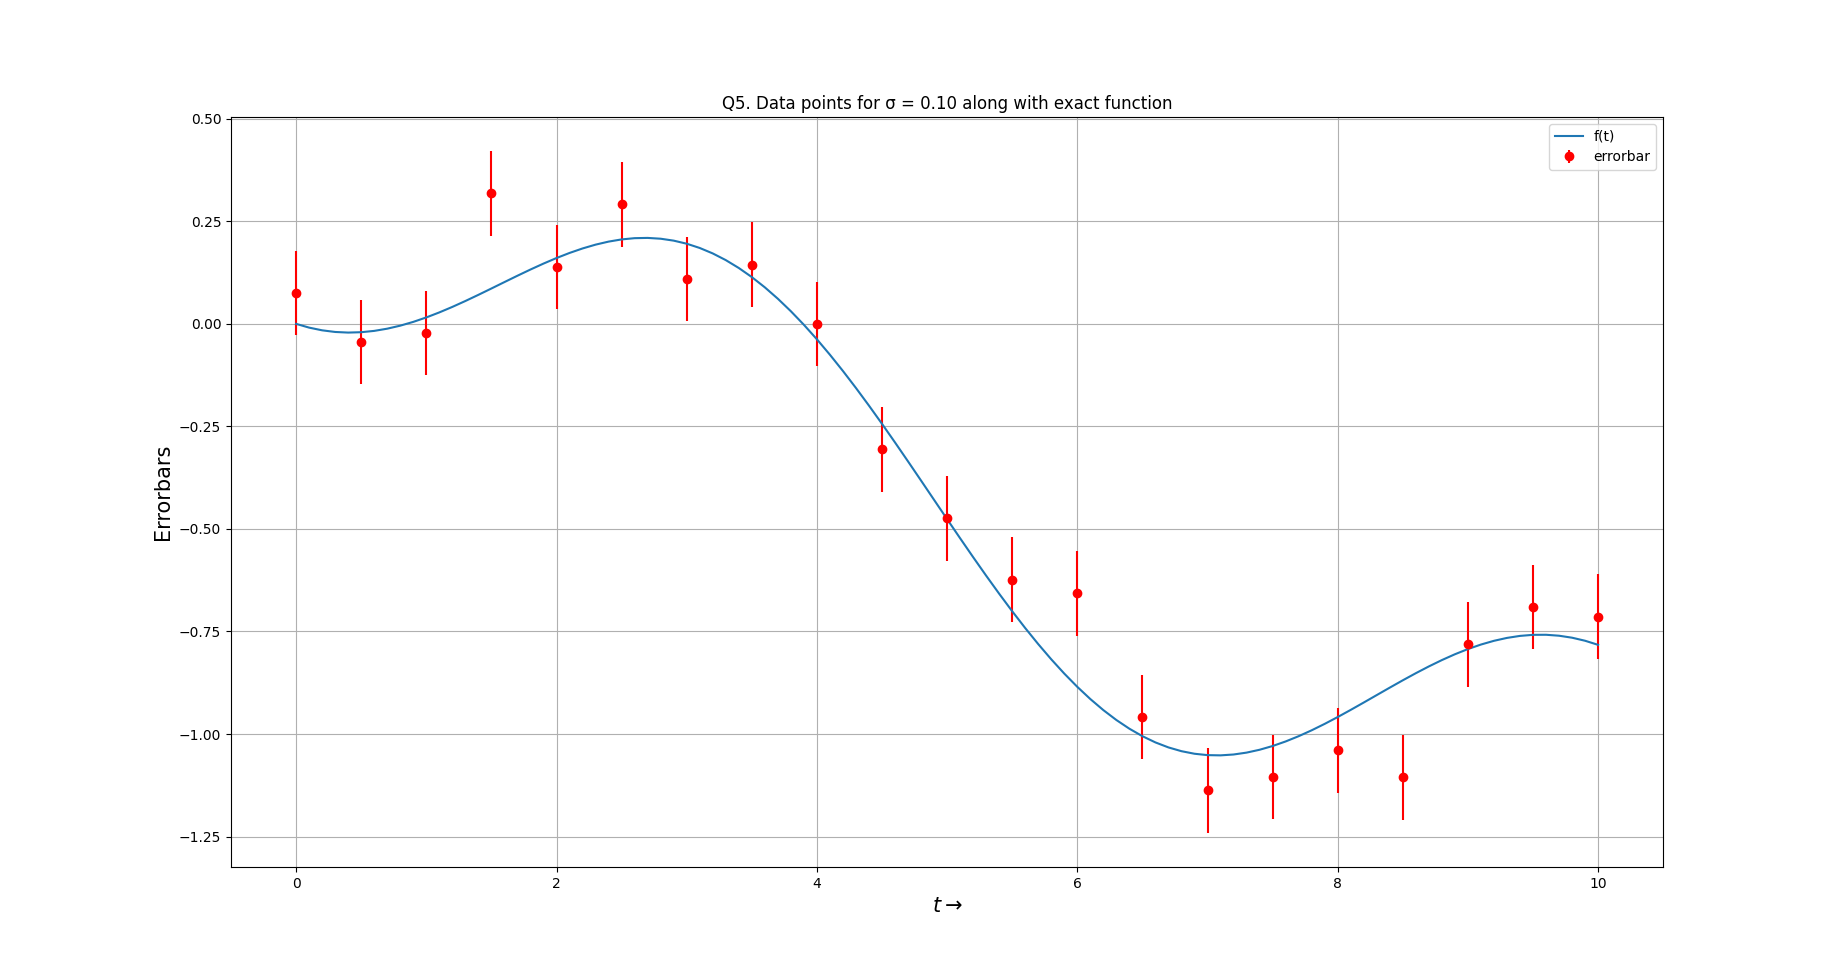
\includegraphics[scale=0.35]{Figure_3.png}
	\caption{Errorbar plot}
	\label{fig:errobars}
\end{figure}

\item Finding the product of $M\cdot p$ and verifying it is equal to $G$. Furthermore, $Mp-G$ is a zero vector, as the output from the python program states:
\begin{psudo}
Verifying Mp - G = 0
[0. 0. 0. 0. 0. 0. 0. 0. 0. 0. 0. 0. 0. 0. 0. 0. 0. 0. 0. 0. 0. 0. 0. 0.
 0. 0. 0. 0. 0. 0. 0. 0. 0. 0. 0. 0. 0. 0. 0. 0. 0. 0. 0. 0. 0. 0. 0. 0.
 0. 0. 0. 0. 0. 0. 0. 0. 0. 0. 0. 0. 0. 0. 0. 0. 0. 0. 0. 0. 0. 0. 0. 0.
 0. 0. 0. 0. 0. 0. 0. 0. 0. 0. 0. 0. 0. 0. 0. 0. 0. 0. 0. 0. 0. 0. 0. 0.
 0. 0. 0. 0. 0.]
\end{psudo}
\begin{figure}[H]
	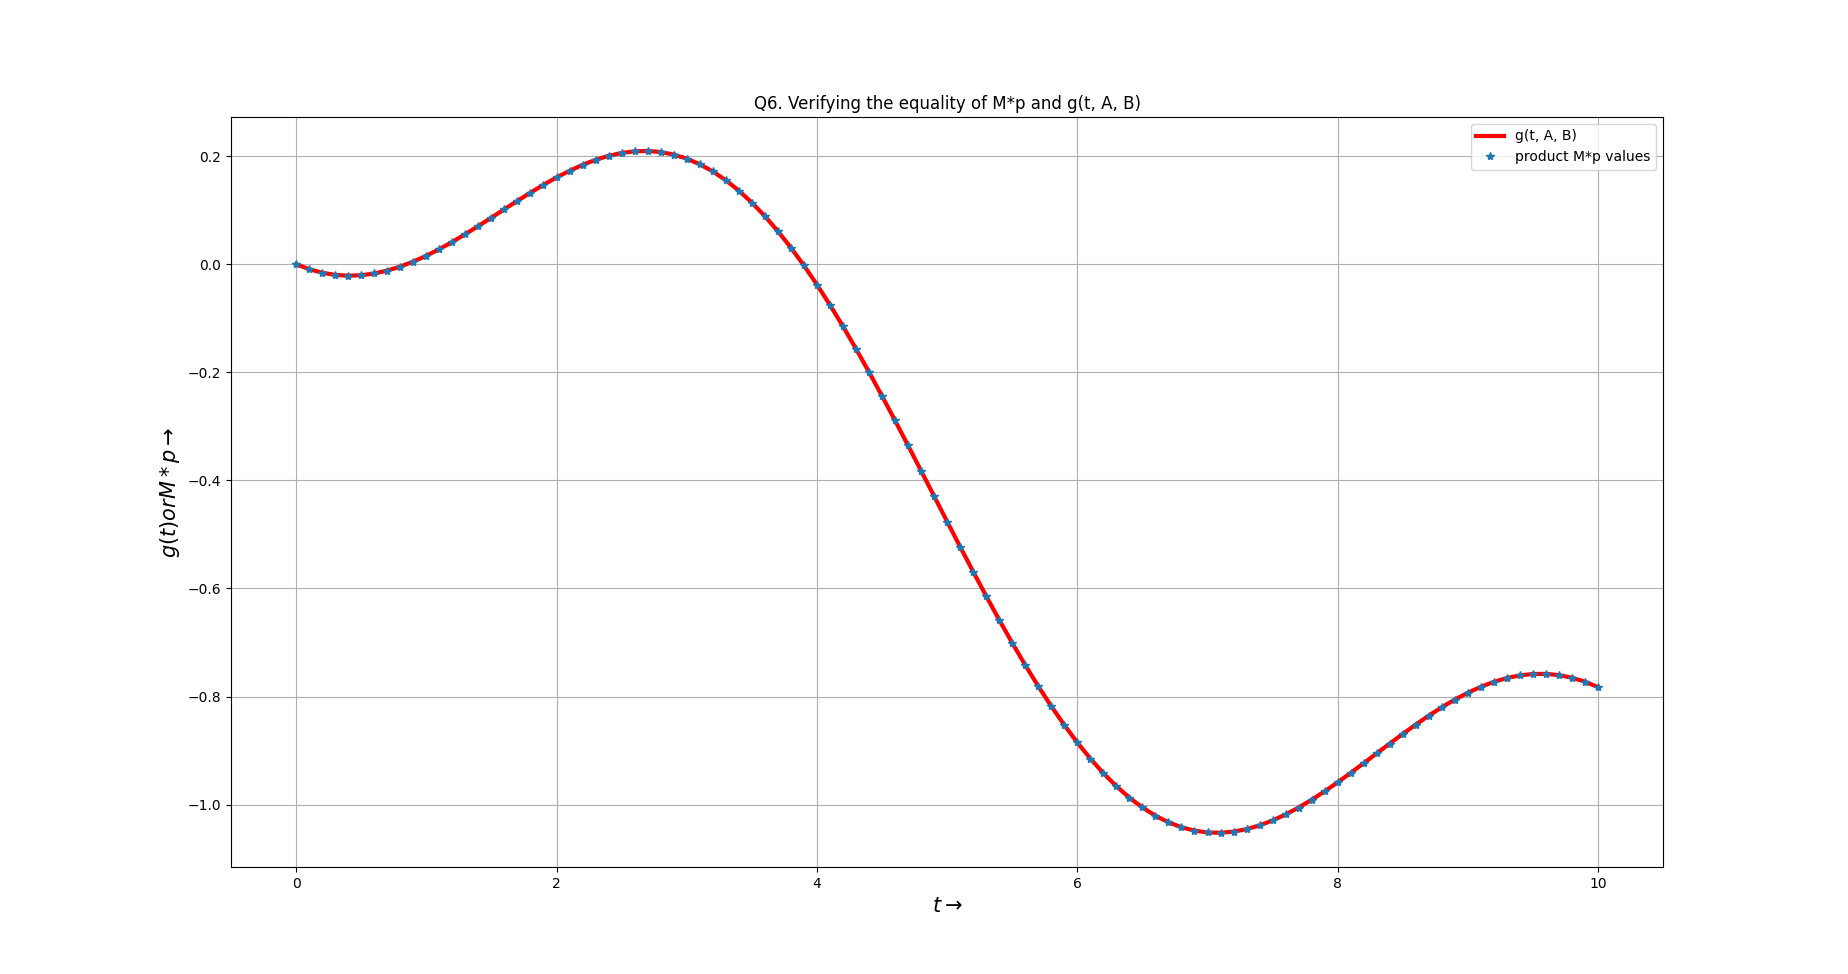
\includegraphics[scale=0.35]{Figure_9.png}
	\caption{Verifying Mp = G via a plot vs $t$}
	\label{fig:contour}
\end{figure}

\item The error $\epsilon_{ij}$ was calculated by two for loops, one for subscript i and j. This implements equation (4) as follows:
\begin{psudo}
E = np.zeros((len(A0), len(B0)))
    f = y[:, i]
    for i in range(len(A0)):
        for j in range(len(B0)):
            E[i, j] = ((f - g(x, A0[i], B0[j]))**2).mean(axis=0)
\end{psudo}
As k goes from 0 to 101, we take the mean of all the values in the numpy array, therefore the summation and division by 101 as in equation (4) is implemented.
\item Contour plot of the mean squared error vs. $A$ and $B$
\begin{figure}[H]
	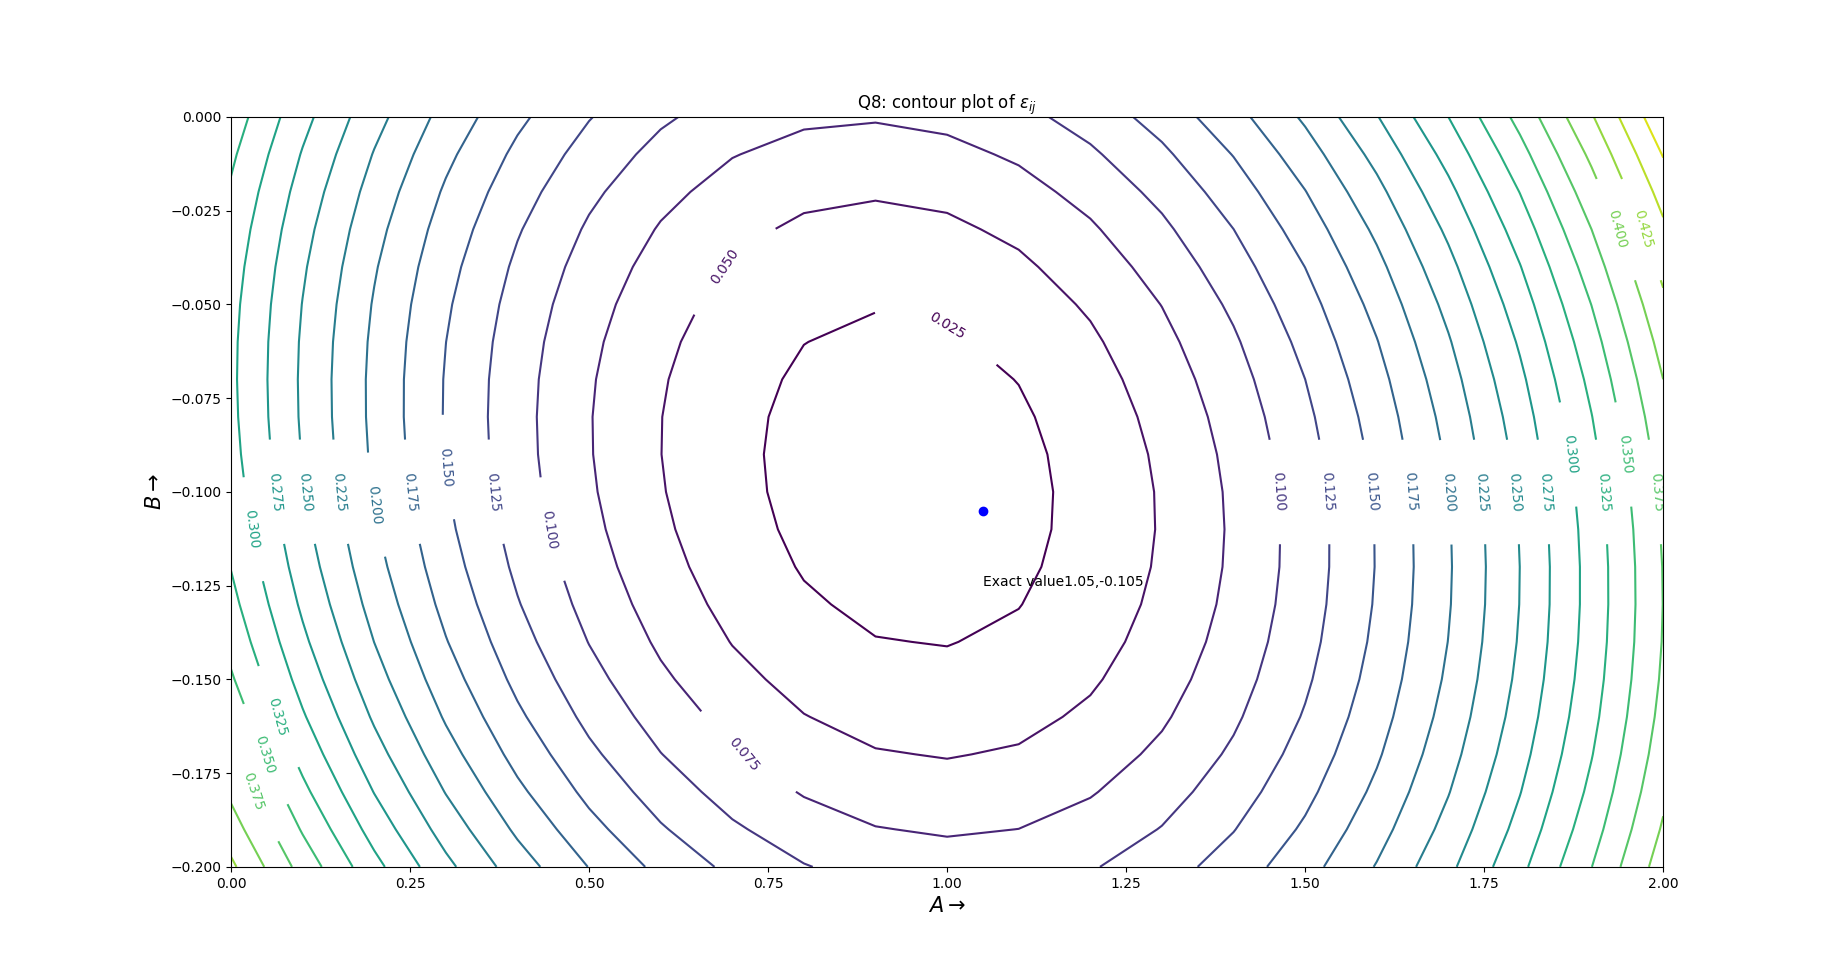
\includegraphics[scale=0.35]{Figure_8.png}
	\caption{Contour Plot of Mean Squared Error vs $A$ and $B$}
	\label{fig:contour}
\end{figure}
the contours appear converge near the exact value (1.05,-0.105), and has only one minima.
\clearpage
\item The variation of error in approximation with the standard deviation of the noise
\begin{figure}[H]
	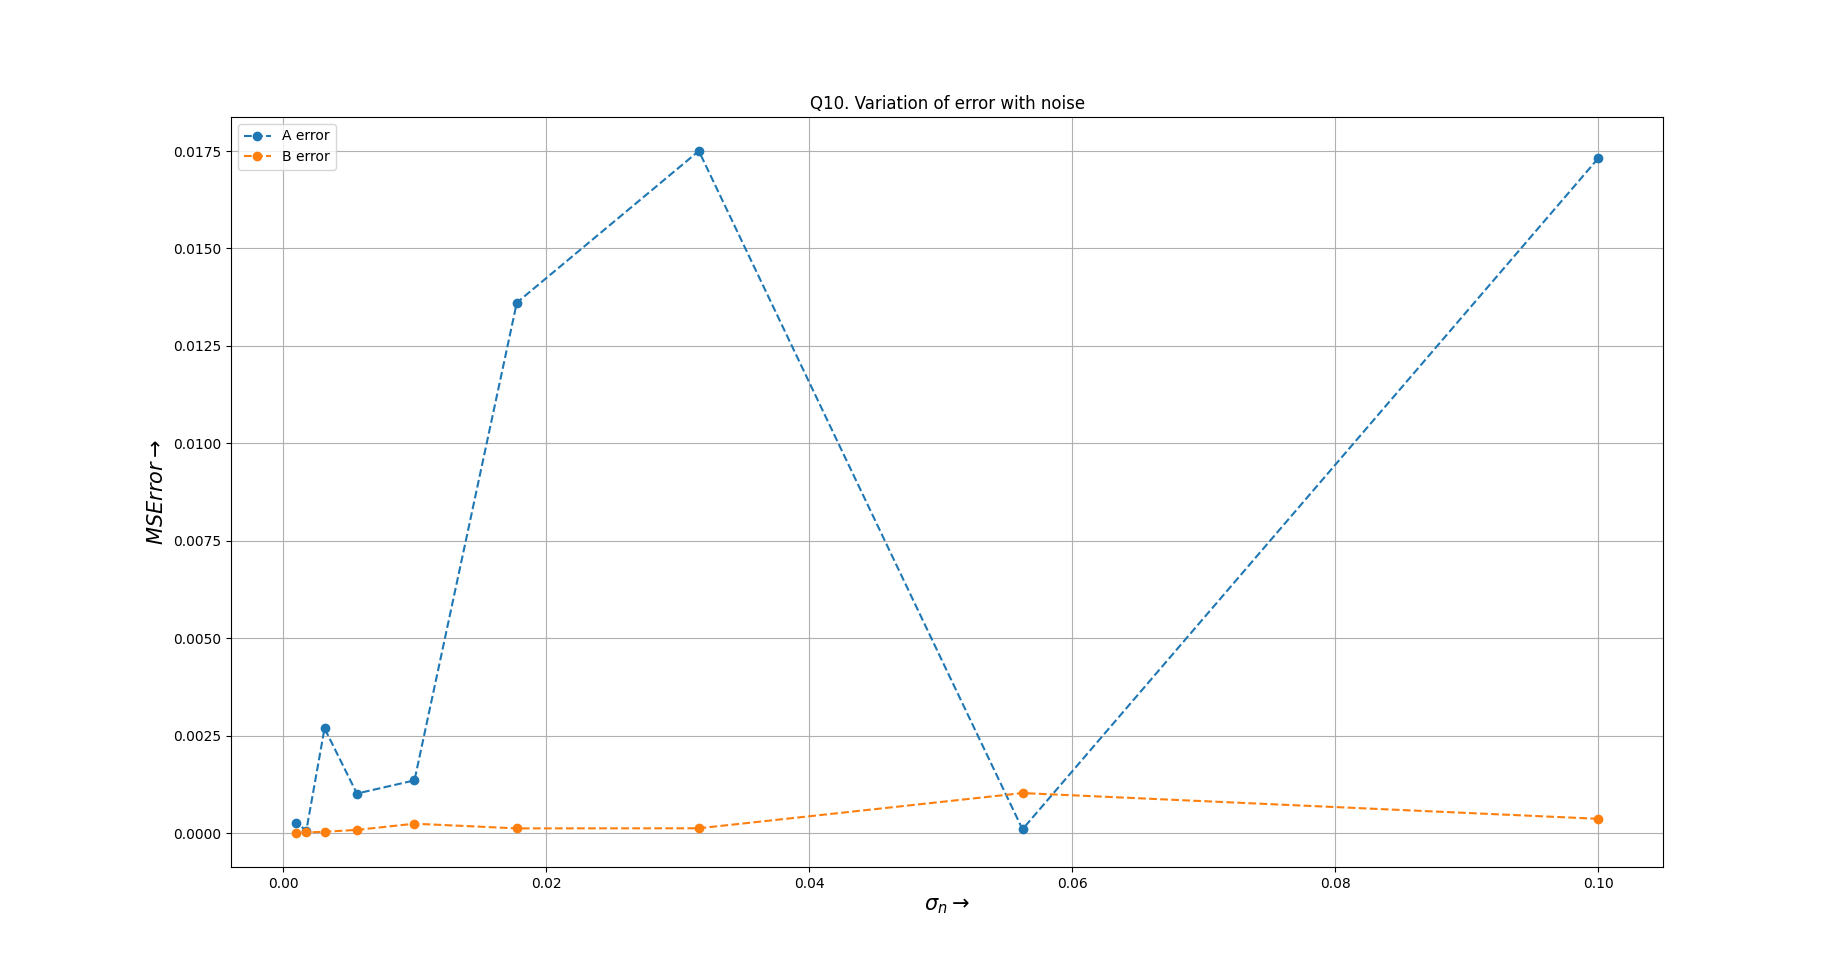
\includegraphics[scale=0.35]{Figure_10.png}
	\caption{Plot for Error in estimation of $A$ and $B$ vs standard deviation in noise}
	\label{fig:eplot}
\end{figure}
As seen in the plot the error in estimation of $A$ increases suddenly with standard deviation of noise, while the error in estimation of $B$ remains nearly constant. 

\item The loglog plot of variation of error in approximation with the standard deviation of the noise
\begin{figure}[H]
	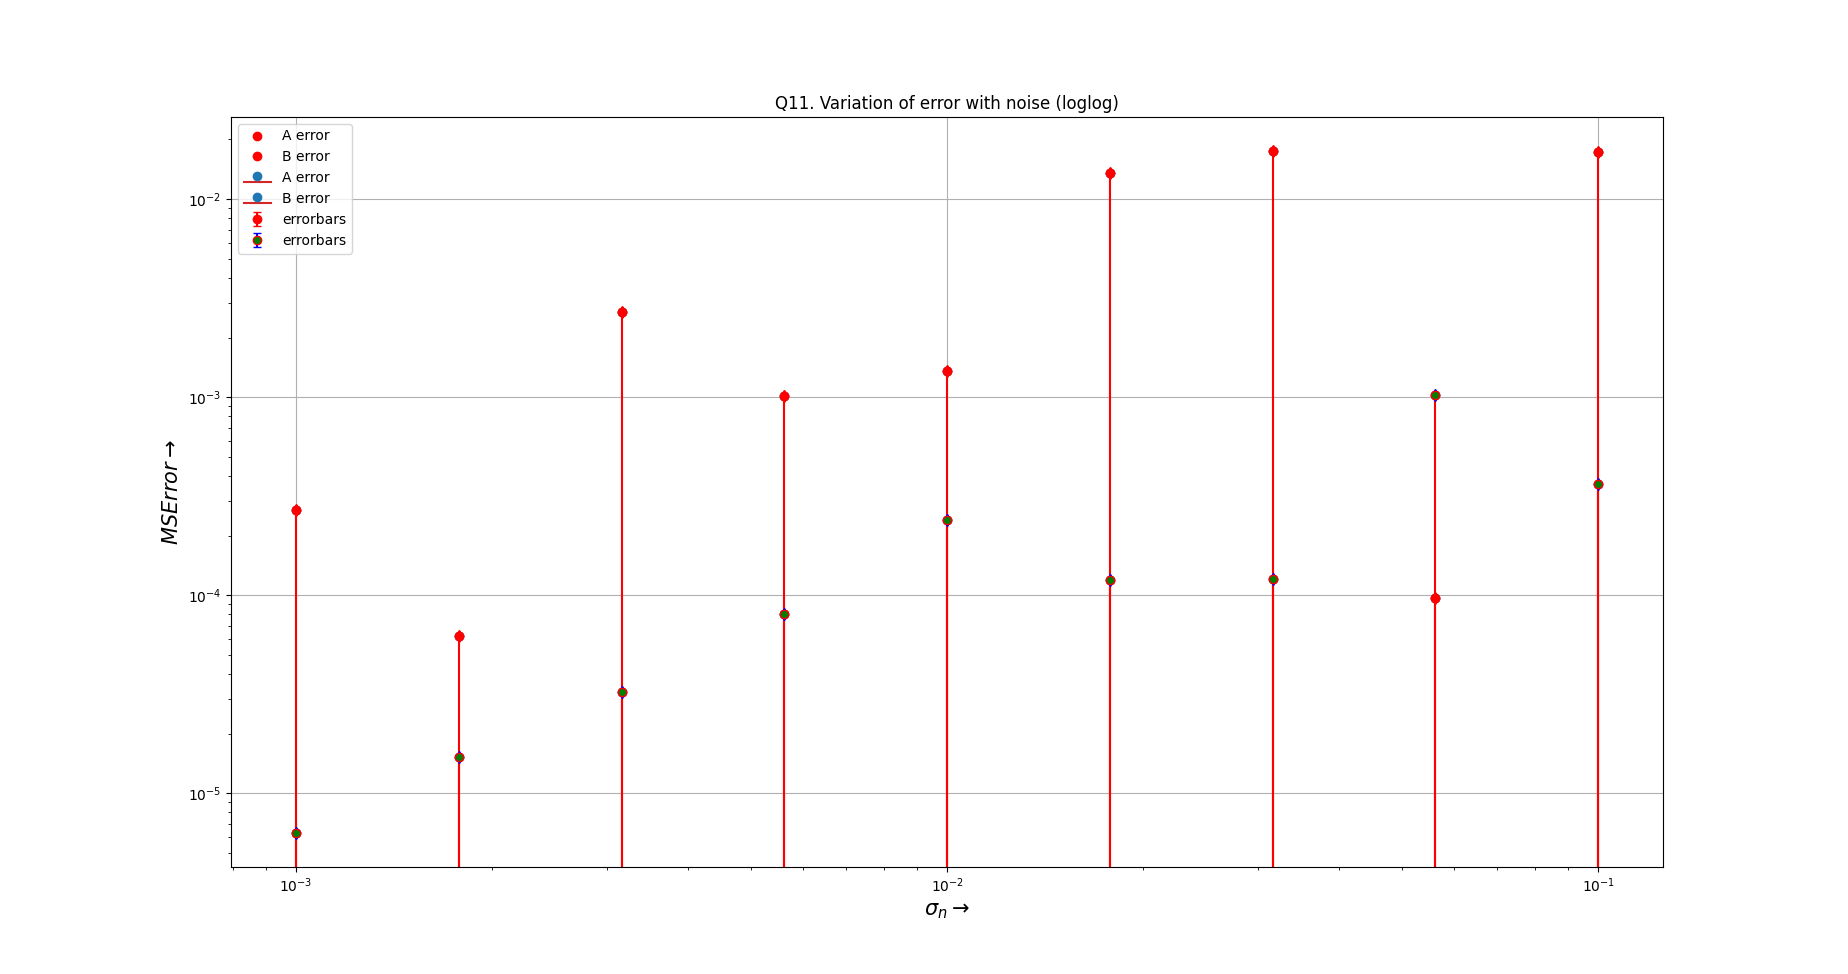
\includegraphics[scale=0.35]{Figure_11.png}
	\caption{log-log Plot for Error in estimation of $A$ and $B$ vs standard deviation in noise}
	\label{fig:logplota}
\end{figure}
As seen in the graph, both error in estimation of $A$ and $B$ show linear dependency on standard deviation of noise.
\end{enumerate}

\subsection*{Conclusions}
By the minimization of Mean Squared Error in the data points using the method of least squares gives a very close estimation of $A$ and $B$. The mean square error is within $2\%$ when the standard deviation is 0.1.\\ \\
The minima of the Mean Squared Error $\epsilon_{ij}$ in the contour plot of equation (4) provides the estimates of $A$ and $B$ for the data.\\ \\
We observe that there is only one minima in the contour plot. This indicates that least squares method has only one optimal solution.\\ \\
By experimenting with noise of varying standard deviations, we obtained the following results about $A$ and $B$:
\begin{itemize}
    \item $B$ varies very little with the standard deviation of noise, while $A$ varies significantly.\\
\item Error in estimating $A$ and $B$ has linear variation with standard deviation of noise in the loglog scale.
\end{itemize}

\end{document}